\graphicspath{{img/ch4}}

\section{Evidence of Cavities Beneath Lunar Pits}

Evidence for subsurface cavities beneath lunar pits is derived from morphological observations, geophysical gravity anomalies, radar sounder reflections, and thermal data. These findings point to large, interconnected voids beneath regions such as \textbf{Marius Hills} and \textbf{Mare Tranquillitatis}, supporting their interpretation as remnants of ancient lava tubes and key features of lunar geological evolution.

\subsection{Morphological Evidence}

Overhanging walls and roof collapses in lunar pits strongly suggest access points to larger subsurface voids, such as intact lava tubes (see Fig. \ref{fig:image1}). High-resolution imagery from the Lunar Reconnaissance Orbiter (LROC) has revealed alignments between these pits and sinuous rilles—ancient lava flow channels associated with underground tubes \citep{lunar-pits-entrances-to-caves, grails-gradients-mariushills}. The Marius Hills region, in particular, shows clear morphological correlations with known volcanic features, as seen in Figure~\ref{fig:marius-hills-collapse}.

\textbf{Collapse Chains and Pit Alignments:} Linear sequences of pits, known as collapse chains, further support the hypothesis of underlying cavities. These chains represent the progressive collapse of lava tube roofs, forming surface depressions that trace the subsurface voids. This is particularly evident in Marius Hills, where pit alignments correlate with surface rilles and lava tubes observed on Earth \citep{new-wagner, cavities-selene-lavatubes}.

\begin{figure}[H]
    \centering
    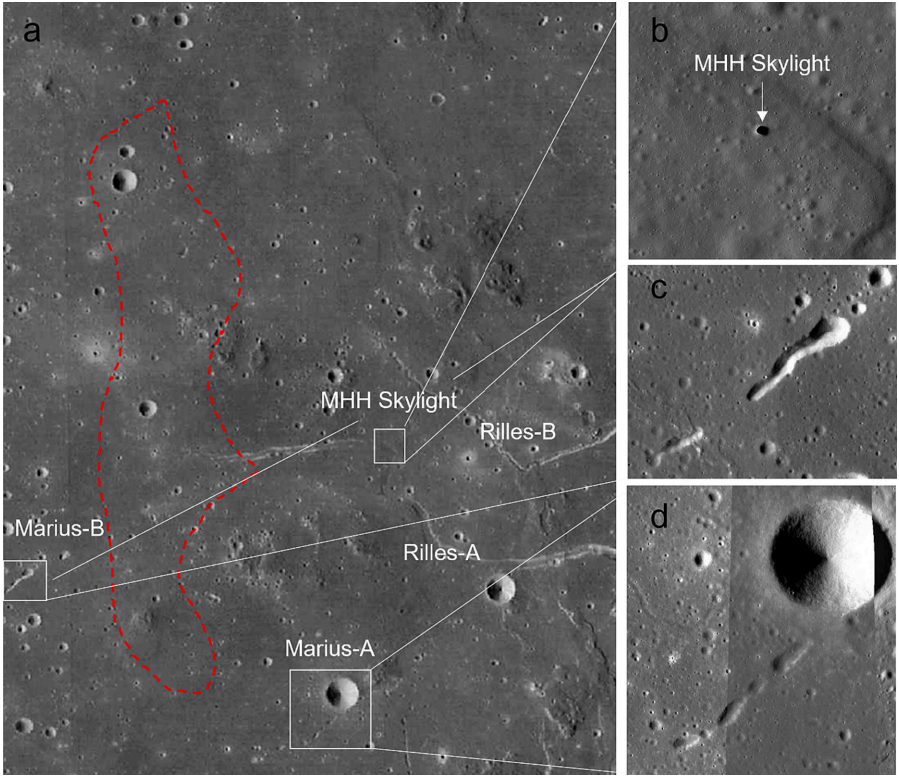
\includegraphics[width=0.5\linewidth]{marius_hills_collapse.png}
    \caption{LROC WAC image of the Marius Hills region, showing collapse chains, sinuous rilles, and skylights. The red dashed line marks the approximate path of the subsurface lava tube. 
    \textbf{(a)} Overview of the Marius Hills region with localized collapse chains and skylights. 
    \textbf{(b)} Close-up of the Marius Hills Hole (MHH). 
    \textbf{(c)} Marius-B collapse chain. 
    \textbf{(d)} Marius-A collapse chain. 
    Adapted from \citet{grails-gradients-mariushills}.}
    \label{fig:marius-hills-collapse}
\end{figure}

\subsection{Geophysical Evidence}

\textbf{Gravity Anomalies from GRAIL:} Subsurface cavities induce detectable gravitational anomalies due to mass deficits in hollow regions. Data from the \textbf{Gravity Recovery and Interior Laboratory (GRAIL)} mission has revealed mass deficits beneath several pit locations. For example, in Marius Hills, Bouguer gravity gradients identified a hollow structure approximately 60 km long and 9 km wide at a depth of 600 m \citep{grails-gradients-mariushills}. These anomalies align closely with pit locations and other volcanic features.

\begin{figure}[H]
    \centering
    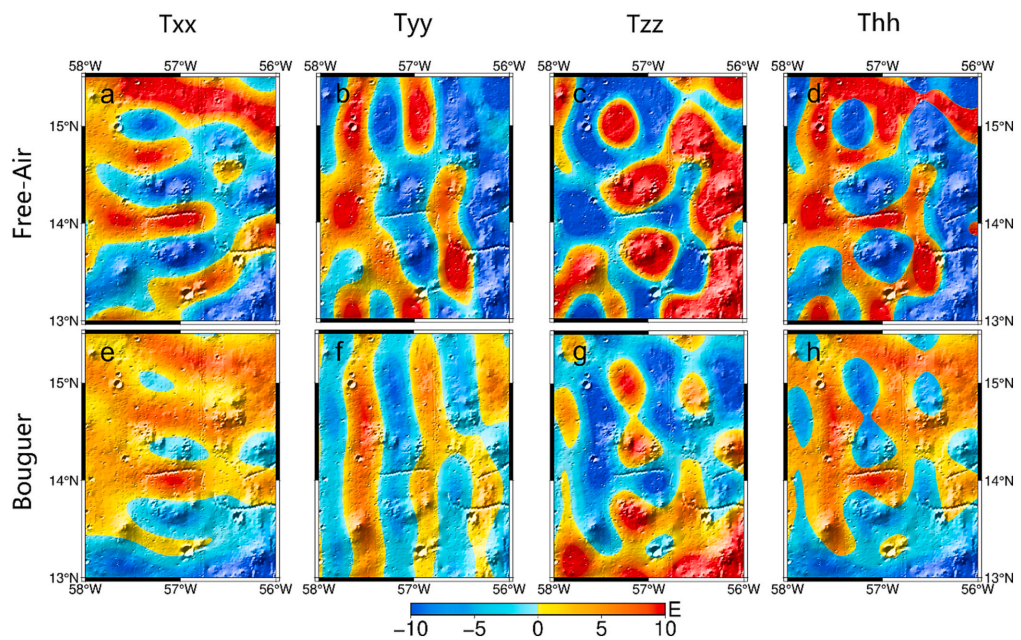
\includegraphics[width=0.85\linewidth]{grail-images-grabity.png}
    \caption{Gravitational anomalies in the Marius Hills region detected by GRAIL. Bouguer gravity gradients reveal mass deficits (blue), indicative of subsurface voids such as intact lava tubes. Adapted from \citet{grails-gradients-mariushills}.}
    \label{fig:marius-hills-gravity}
\end{figure}

\subsection{Radar Evidence from SELENE and Mini-RF}

\textbf{Radar Echoes from SELENE (Kaguya):} Radar sounders like the Lunar Radar Sounder (LRS) onboard SELENE have been instrumental in confirming subsurface cavities. Double-echo patterns—secondary radar reflections—indicate voids beneath the lunar surface. At Mare Tranquillitatis, LRS data suggest a subsurface cavity extending several kilometers \citep{cavities-selene-lavatubes}.

\begin{figure}[H]
    \centering
    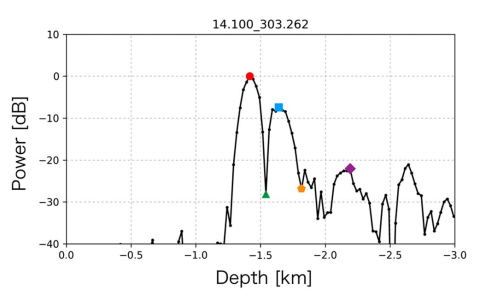
\includegraphics[width=0.35\linewidth]{selene-doublebump.png}
    \caption{SELENE LRS radar echoes showing a characteristic double-echo pattern indicative of a subsurface void. The first peak represents the surface reflection, while the second peak corresponds to the void floor. Adapted from \citep{cavities-selene-lavatubes}.}
    \label{fig:radar-echoes}
\end{figure}

\textbf{Mini-RF Contributions:} Using Mini-RF data, Carrer et al. (2024) identified radar reflections beyond the walls of Mare Tranquillitatis Pit. These reflections are consistent with a lava tube connected to the pit. Combined with gravitational and morphological data, this strengthens the hypothesis of intact subsurface voids \citep{Carrer2024}.

\begin{figure}[H]
    \centering
    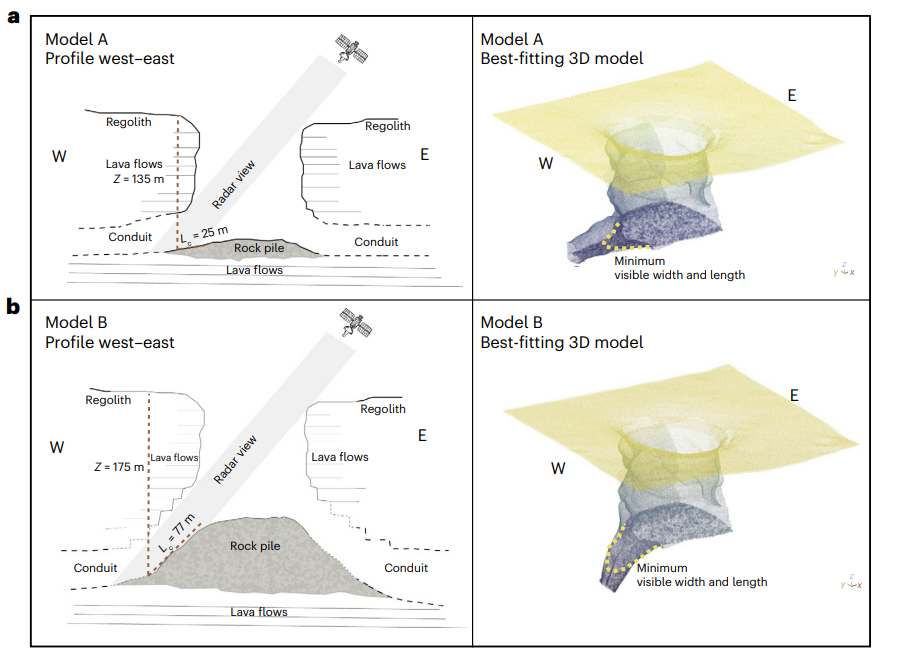
\includegraphics[width=0.85\linewidth]{carrer-renders.png}
    \caption{Reconstructed Mare Tranquillitatis Pit (MTP) cave conduit based on inversion of Mini-RF radar data. \textbf{(a)} Model A with a conduit of approximately 135 m width and a low floor slope. \textbf{(b)} Model B with a conduit approximately 175 m wide and steeper floor slopes. The 3D models show the surface (yellow), subsurface lava flows (blue), and inferred lava tube conduit (gray). Adapted from \citep{Carrer2024}.}
    \label{fig:mtp-cave-conduit}
\end{figure}

\subsection{Thermal Observations as Indirect Evidence}

Thermal data also suggest subsurface cavities beneath pits. The Diviner Lunar Radiometer Experiment has shown that the interiors of pits maintain stable temperatures, supporting the idea of thermally buffered environments consistent with underground voids. For example, temperatures within the Mare Tranquillitatis pit remain near -25°C throughout the lunar night, suggesting limited thermal exposure due to cavity geometry \citep{thermal-lunar-pits, newer-thermal}.

This stability aligns with the blackbody cavity effect, where limited exposure to sunlight and the insulating properties of surrounding rock create stable conditions. Such environments could provide ideal conditions for exploration and resource utilization.